\chapter{Resultados e Discussão}

Este capítulo apresenta os resultados dos parâmetros calculados para a Equação \ref{eq:equacao-geral}. Para isso, foi desenvolvido um código computacional, desenvolvido em Python 3.2, implementando a teoria apresentada nos capítulos anteriores. Também é apresentado o desempenho obtido pela arquitetura de rede neural artificial estudada. 

\section{Resultados para o modelo estatístico}

Os registros da cidade de Recife foram colocados em sequência cronológica de segundos. Posteriormente, selecionaram-se as máximas precipitações anuais por duração, sempre verificando se estavam de acordo com os critérios estabelecidos no capítulo anterior. A Tabela \ref{tab:precipitacoes-recife} exibe as precipitações selecionadas para cada duração entre os anos de 2003 e 2011.

%precipitação máxima
\begin{table}[h]
\caption{Precipitações máximas para a cidade de Recife}
\begin{tabular}{ccccccccccc}
\toprule
\centering
Ano & \multicolumn{10}{c}{Duração (min)}                                                  \\ \cline{2-11} 
     & 5     & 10    & 15    & 30    & 60    & 120    & 240    & 360    & 720    & 1080   \\ \hline
2003 & 8     & 14,25 & 16,5  & 22,25 & 29,25 & 36,5   & 50,75  & 61,5   & 94,25  & 100,25 \\
2004 & 8     & 11,5  & 16,5  & 29,5  & 45,25 & 52,25  & 53,5   & 54     & 81     & 90,25  \\
2005 & 17,25 & 29,25 & 36,5  & 51,25 & 69,75 & 102,25 & 137,25 & 176,75 & 206,5  & 206,5  \\
2006 & 8,75  & 13,25 & 17,5  & 29    & 45,25 & 62,25  & 71,5   & 93,25  & 102,75 & 102,75 \\
2007 & 9,5   & 13    & 17,25 & 26,75 & 40,5  & 41,75  & 47,25  & 56     & 73,75  & 80,75  \\
2008 & 11    & 20,5  & 28    & 41,75 & 63    & 66,5   & 68,75  & 86     & 111,25 & 112,75 \\
2009 & 9,25  & 15,5  & 20,25 & 37,75 & 47,5  & 55,5   & 82     & 97,25  & 110,5  & 112,5  \\
2010 & 9,75  & 16,5  & 20,75 & 26    & 33,25 & 44,5   & 77,75  & 95     & 112    & 125    \\
2011 & 12,25 & 24    & 32,5  & 57    & 71,25 & 87,25  & 100,75 & 102    & 124,75 & 125,75 \\ \bottomrule
\end{tabular}
\fonte{Autores}
\label{tab:precipitacoes-recife}
\end{table}

%gumbel
As intensidades máximas anuais calculadas por meio da distribuição de probabilidade de Gumbel para máximos podem ser visualizadas na Tabela \ref{tab:gumbel}.


\begin{table}[h]
\centering
\caption{Intensidades em mm/h para distribuição de Gumbel}
\begin{tabular}{@{}cccccccccc@{}}
\toprule
\multirow{2}{*}{\begin{tabular}[c]{@{}l@{}}Duração\\ (min)\end{tabular}} & \multicolumn{9}{c}{Período de Retorno (anos)} \\ \cmidrule(l){2-10} 
  & 2      & 3      & 5      & 10     & 15     & 20     & 25     & 50     & 100    \\ \midrule
5 & 119,27 & 133,84 & 150,07 & 170,45 & 181,96 & 190,01 & 196,21 & 215,32 & 234,29 \\
10 & 99,34  & 114,16 & 130,65 & 151,39 & 163,08 & 171,27 & 177,58 & 197,01 & 216,30 \\
15 & 86,47  & 99,12  & 113,20 & 130,90 & 140,89 & 147,88 & 153,26 & 169,85 & 186,32 \\
30 & 67,41  & 77,54  & 88,82  & 102,99 & 110,99 & 116,59 & 120,90 & 134,19 & 147,38 \\
60 & 46,94  & 53,31  & 60,41  & 69,33  & 74,36  & 77,89  & 80,60  & 88,96  & 97,26  \\
120 & 28,70  & 33,24  & 38,29  & 44,64  & 48,23  & 50,74  & 52,67  & 58,62  & 64,53  \\
240 & 17,99  & 20,95  & 24,25  & 28,40  & 30,75  & 32,38  & 33,65  & 37,54  & 41,40  \\
360 & 14,20  & 16,79  & 19,67  & 23,28  & 25,33  & 26,76  & 27,86  & 31,25  & 34,62  \\
720 & 8,89   & 10,23  & 11,73  & 13,61  & 14,67  & 15,41  & 15,98  & 17,75  & 19,50  \\
1080 & 6,19   & 7,04   & 7,98   & 9,17   & 9,84   & 10,31  & 10,67  & 11,79  & 12,89  \\ \bottomrule
\end{tabular}
\fonte{Autores}
\label{tab:gumbel}
\end{table}

Apesar das séries de máximas precipitações anuais possuírem um intervalo de dados inferior ao recomendado pela literatura (de 30 anos), o resultado do Teste de Kolmogorov-Smirnov indica que essas amostras são representativas das precipitações extremas. Ainda que o Teste de Kolmogorov-Smirnov torna-se mais rigoroso para níveis de significância superiores a 20\%, não se pode rejeitar a hipótese de que a distribuição estatística escolhida (distribuição de Gumbel) representa as chuvas para a região em estudo.
O coeficiente de determinação ficou entre o intervalo de 0,89624 e 0,98455 para todas as durações estudadas. Os valores desses coeficientes legitimam a aderência da distribuição de Gumbel aos dados dessa região. A Tabela \ref{tab:teste-de-ks} exibe um resumo dos testes realizados. 

\begin{table}[h]
\centering
\caption{Resultados do teste de aderência para o teste de Kolmogorov-Smirnov}
\begin{tabular}{@{}cccccccc@{}}
\toprule
\multirow{2}{*}{\begin{tabular}[c]{@{}c@{}}Duração\\ (min)\end{tabular}} & \multirow{2}{*}{\begin{tabular}[c]{@{}c@{}}Divergência \\ Máxima\end{tabular}} & \multicolumn{4}{c}{\begin{tabular}[c]{@{}c@{}}Valores do teste de KS com n=9\\ Nível de significância:\end{tabular}} & \multirow{2}{*}{\begin{tabular}[c]{@{}c@{}}Passa no\\ Teste KS?\end{tabular}} & \multirow{2}{*}{Ajuste R2} \\ \cmidrule(lr){3-6}
             &      & 20\%    & 10\%    & 5\%     & 1\%    &     &        \\ \midrule
5            & 0,1289             & 0,3390  & 0,3880  & 0,4320  & 0,5140 & Sim & 0,93677      \\
10           & 0,1516             & 0,3390  & 0,3880  & 0,4320  & 0,5140 & Sim & 0,95283      \\
15           & 0,1605             & 0,3390  & 0,3880  & 0,4320  & 0,5140 & Sim & 0,89624      \\
30           & 0,1315             & 0,3390  & 0,3880  & 0,4320  & 0,5140 & Sim & 0,95010      \\
60           & 0,0880             & 0,3390  & 0,3880  & 0,4320  & 0,5140 & Sim & 0,95730      \\
120          & 0,0968             & 0,3390  & 0,3880  & 0,4320  & 0,5140 & Sim & 0,98455      \\
240          & 0,1213             & 0,3390  & 0,3880  & 0,4320  & 0,5140 & Sim & 0,97272      \\
360          & 0,1396             & 0,3390  & 0,3880  & 0,4320  & 0,5140 & Sim & 0,91924      \\
720          & 0,1418             & 0,3390  & 0,3880  & 0,4320  & 0,5140 & Sim & 0,93415      \\
1080         & 0,1033             & 0,3390  & 0,3880  & 0,4320  & 0,5140 & Sim & 0,92950 \\ \bottomrule
\end{tabular}
\fonte{Autores}
\label{tab:teste-de-ks}
\end{table}

Após a validação da distribuição estatística os valores dos coeficientes $k$, $a$, $b$ e $c$, foram determinados por meio de regressão linear múltipla. Os parâmetros finais para esses coeficientes são representados pela Equação \ref{eq:idf-recife}.

%eq chuva intensa
\begin{equation}
    i = \frac{1380,2176\times T_r^{0,19369}}{(t+22)^{0,78201}}
\label{eq:idf-recife}
\end{equation}

De posse dos coeficientes que melhor se ajustaram à distribuição escolhida é possível montar a família de curvas que representam a intensidade máxima de chuva para cada período de retorno em função da duração. A Figura \ref{fig:idf-ajustada} representa as oito curvas que correlacionam intensidade-duração-frequência para a cidade de Recife.

\begin{figure}[h]
    \caption{Curvas IDF ajustadas para a cidade de Recife}
    \centering
    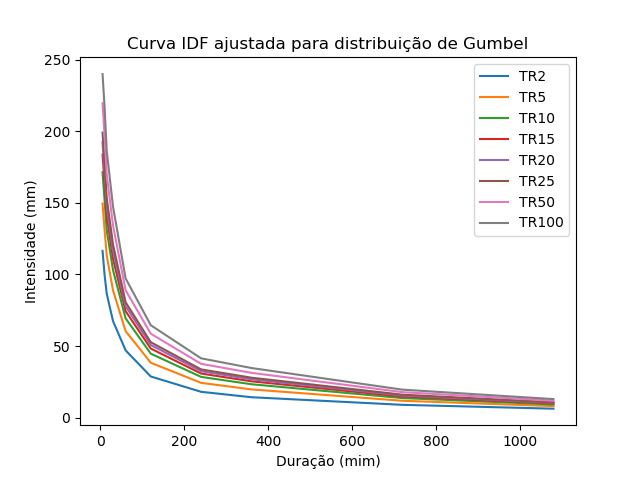
\includegraphics[width=0.8\textwidth]{Textuais/Figuras/curvas-idf-ajustadas.png}
    \fonte{Autores}
    \label{fig:idf-ajustada}
\end{figure}

%rede
\section{Resultados para o modelo de inteligência artificial}

As Figuras \ref{fig:tr2-1n} a \ref{fig:tr100-10n} ilustram as curvas ajustadas para cada período de retorno variando a quantidade de neurônios artificias de 1, 2, 5 e 10 neurônios. Pode-se observar, que a medida em que a quantidade de neurônios é incrementada a saída da rede neural está cada vez mais próxima das intensidades calculadas pela distribuição de Gumbel.

A Tabela \ref{tab:resumo} mostra um resumo dos coeficientes de determinação para cada modelo desse trabalho. Pode-se observar que os valores encontrados pela rede neural estão muito mais próximos da realidade, obtendo uma equação que representa de uma forma mais exata a região de Recife.

\begin{table}[h]
\centering
\caption{Resumo dos coeficientes de determinação para a rede estudada}
\begin{tabular}{@{}ccccccccc@{}}
\toprule
\begin{tabular}[c]{@{}c@{}}Número de \end{tabular} & \multicolumn{8}{c}{Período de Retorno} \\ \cmidrule(l){2-9} 
Neurônios   & 2      & 5      & 10     & 15     & 20     & 25     & 50     & 100    \\ \midrule
1  & 0,9789 & 0,9687 & 0,9654 & 0,9754 & 0,9562 & 0,9658 & 0,9812 & 0,9612 \\
2  & 0,9892 & 0,9756 & 0,9658 & 0,9654 & 0,9654 & 0,9658 & 0,9881 & 0,9781 \\
5  & 0,9951 & 0,9878 & 0,9745 & 0,9851 & 0,9874 & 0,9781 & 0,9956 & 0,9785 \\
10 & 0,9967 & 0,9973 & 0,9856 & 0,9914 & 0,9881 & 0,9789 & 0,9961 & 0,9965 \\ \bottomrule
\end{tabular}
\label{tab:resumo}
\fonte{Autores}
\end{table}

%TR 2
\begin{figure}[h]
    \caption{Curva ajustada para os dados para TR 2 anos e 1 neurônio artificial}
    \centering
    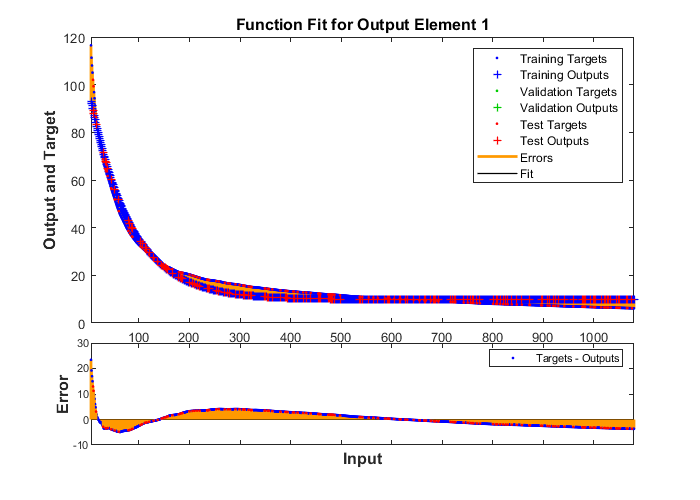
\includegraphics[width=0.74\textwidth]{Textuais/Figuras/NN/tr2-1neuronio.png}
    \fonte{Autores}
    \label{fig:tr2-1n}
\end{figure}

\begin{figure}[h]
    \caption{Curva ajustada para os dados para TR 2 anos e 2 neurônios artificiais}
    \centering
    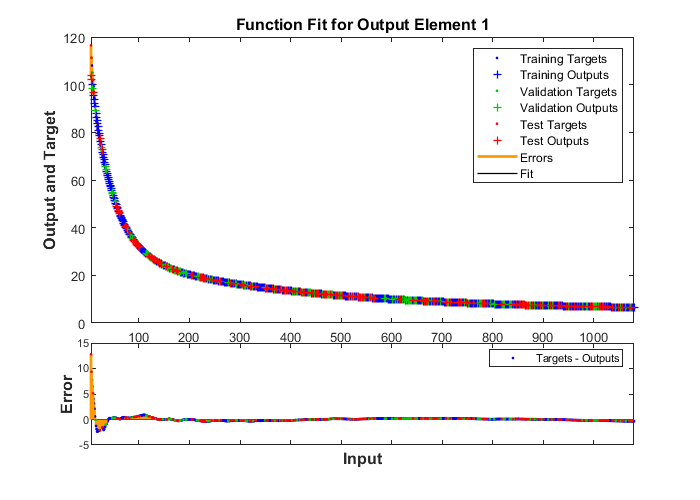
\includegraphics[width=0.74\textwidth]{Textuais/Figuras/NN/tr2-2neuronio.png}
    \fonte{Autores}
    \label{fig:tr2-2n}
\end{figure}

\begin{figure}[h]
    \caption{Curva ajustada para os dados para TR 2 anos e 5 neurônios artificiais}
    \centering
    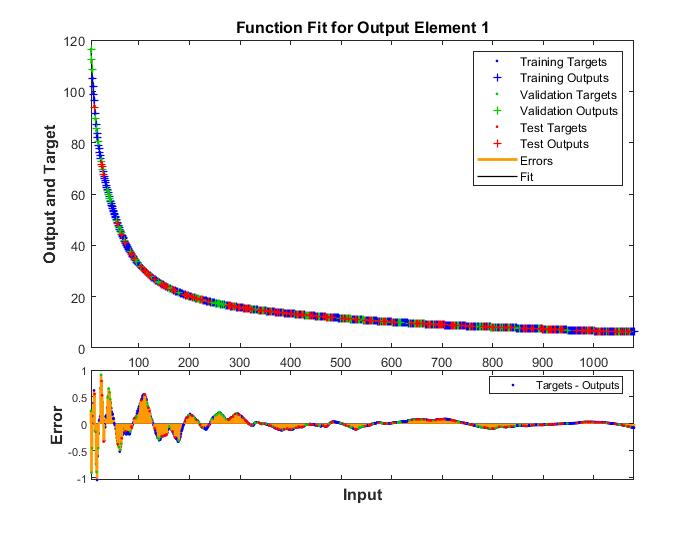
\includegraphics[width=0.74\textwidth]{Textuais/Figuras/NN/tr2-5neuronio.png}
    \fonte{Autores}
    \label{fig:tr2-5n}
\end{figure}

\begin{figure}[h]
    \caption{Curva ajustada para os dados para TR 2 anos e 10 neurônios artificiais}
    \centering
    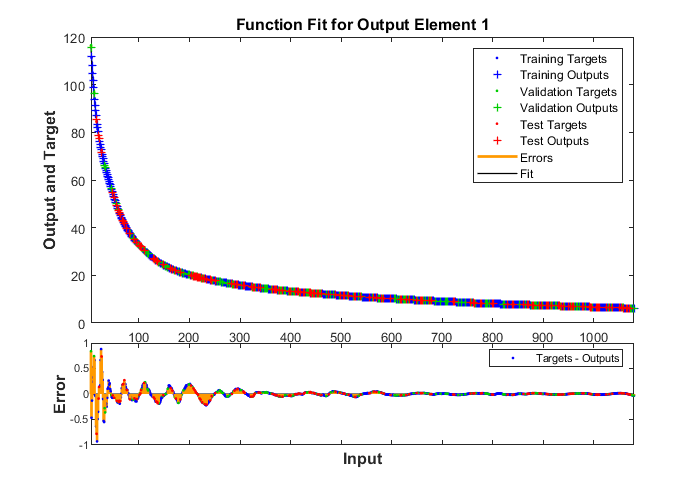
\includegraphics[width=0.74\textwidth]{Textuais/Figuras/NN/tr2-10neuronio.png}
    \fonte{Autores}
    \label{fig:tr2-10n}
\end{figure}
%FIM TR 2

%TR 3
\begin{figure}[h]
    \caption{Curva ajustada para os dados para TR 3 anos e 1 neurônio artificial}
    \centering
    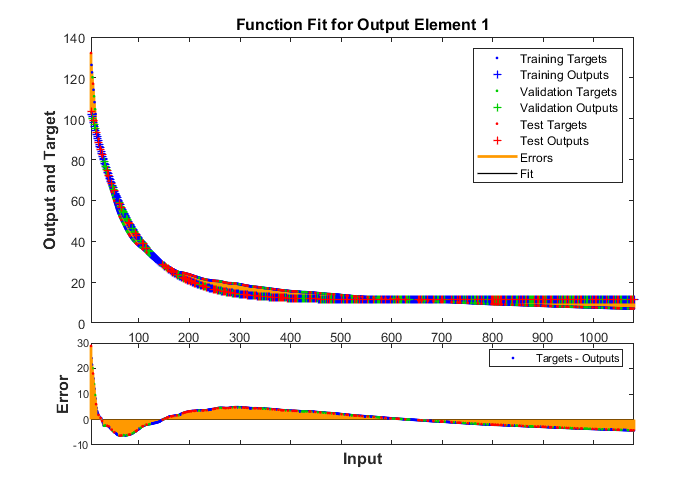
\includegraphics[width=0.74\textwidth]{Textuais/Figuras/NN/tr3-1neuronio.png}
    \fonte{Autores}
    \label{fig:tr3-1n}
\end{figure}

\begin{figure}[h]
    \caption{Curva ajustada para os dados para TR 3 anos e 2 neurônios artificiais}
    \centering
    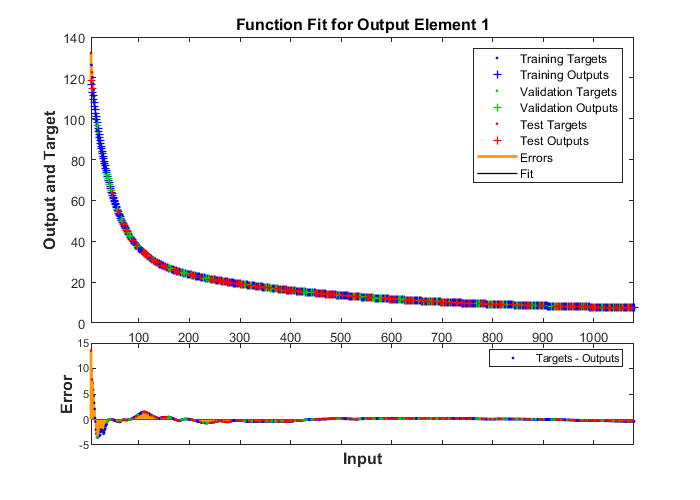
\includegraphics[width=0.74\textwidth]{Textuais/Figuras/NN/tr3-2neuronio.png}
    \fonte{Autores}
    \label{fig:tr3-2n}
\end{figure}

\begin{figure}[h]
    \caption{Curva ajustada para os dados para TR 3 anos e 5 neurônios artificiais}
    \centering
    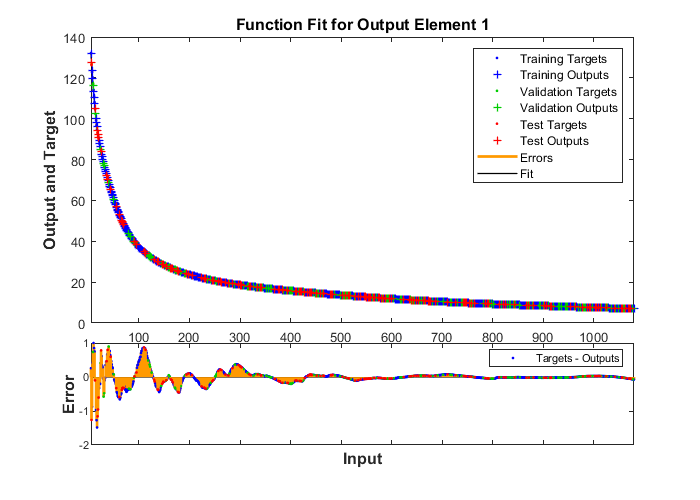
\includegraphics[width=0.74\textwidth]{Textuais/Figuras/NN/tr3-5neuronio.png}
    \fonte{Autores}
    \label{fig:tr3-5n}
\end{figure}

\begin{figure}[h]
    \caption{Curva ajustada para os dados para TR 3 anos e 10 neurônios artificiais}
    \centering
    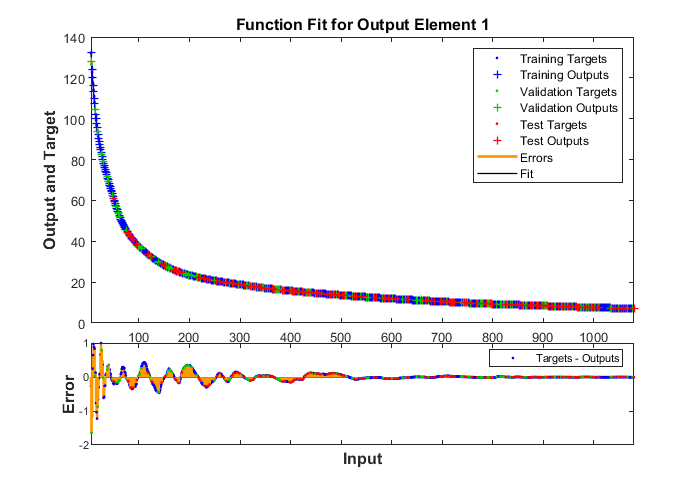
\includegraphics[width=0.74\textwidth]{Textuais/Figuras/NN/tr3-10neuronio.png}
    \fonte{Autores}
    \label{fig:tr3-10n}
\end{figure}
%FIM TR 3

%TR 5
\begin{figure}[h]
    \caption{Curva ajustada para os dados para TR 5 anos e 1 neurônio artificial}
    \centering
    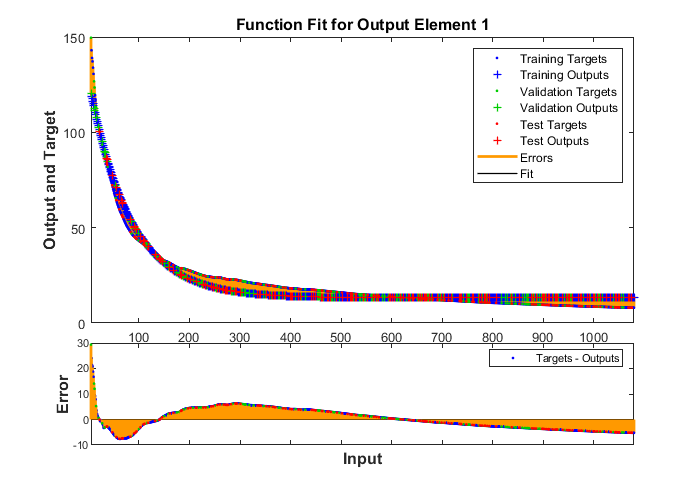
\includegraphics[width=0.74\textwidth]{Textuais/Figuras/NN/tr5-1neuronio.png}
    \fonte{Autores}
    \label{fig:tr5-1n}
\end{figure}

\begin{figure}[h]
    \caption{Curva ajustada para os dados para TR 5 anos e 2 neurônios artificiais}
    \centering
    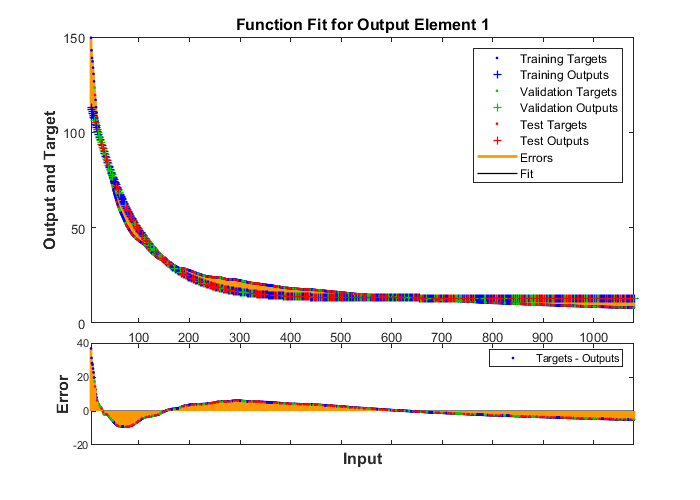
\includegraphics[width=0.74\textwidth]{Textuais/Figuras/NN/tr5-2neuronio.png}
    \fonte{Autores}
    \label{fig:tr5-2n}
\end{figure}

\begin{figure}[h]
    \caption{Curva ajustada para os dados para TR 5 anos e 5 neurônios artificiais}
    \centering
    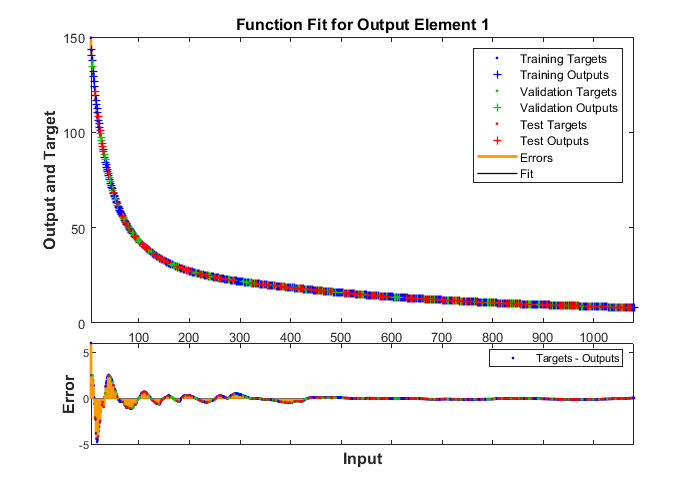
\includegraphics[width=0.74\textwidth]{Textuais/Figuras/NN/tr5-5neuronio.png}
    \fonte{Autores}
    \label{fig:tr5-5n}
\end{figure}

\begin{figure}[h]
    \caption{Curva ajustada para os dados para TR 5 anos e 10 neurônios artificiais}
    \centering
    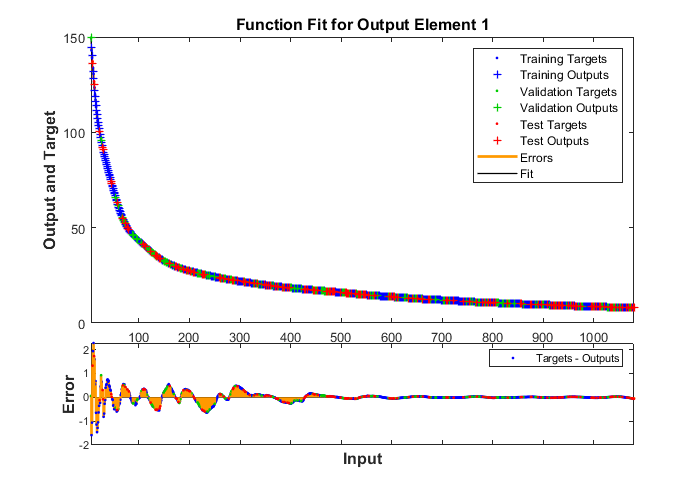
\includegraphics[width=0.74\textwidth]{Textuais/Figuras/NN/tr5-10neuronio.png}
    \fonte{Autores}
    \label{fig:tr5-10n}
\end{figure}
%FIM TR 5

%TR 10
\begin{figure}[h]
    \caption{Curva ajustada para os dados para TR 10 anos e 1 neurônio artificial}
    \centering
    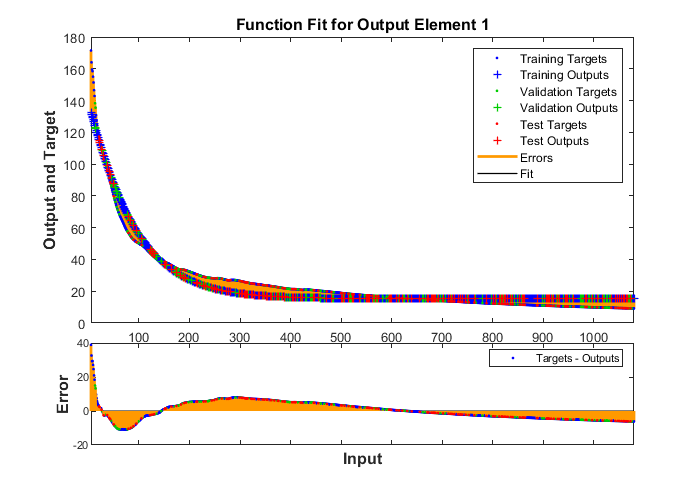
\includegraphics[width=0.74\textwidth]{Textuais/Figuras/NN/tr10-1neuronio.png}
    \fonte{Autores}
    \label{fig:tr10-1n}
\end{figure}

\begin{figure}[h]
    \caption{Curva ajustada para os dados para TR 10 anos e 2 neurônios artificiais}
    \centering
    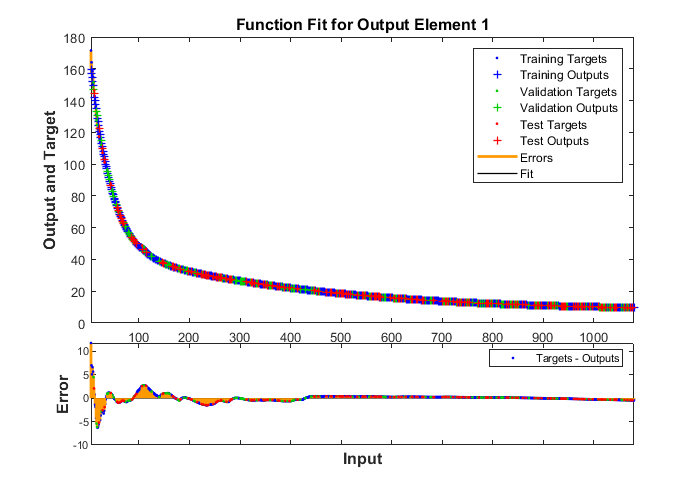
\includegraphics[width=0.74\textwidth]{Textuais/Figuras/NN/tr10-2neuronio.png}
    \fonte{Autores}
    \label{fig:tr10-2n}
\end{figure}

\begin{figure}[h]
    \caption{Curva ajustada para os dados para TR 10 anos e 5 neurônios artificiais}
    \centering
    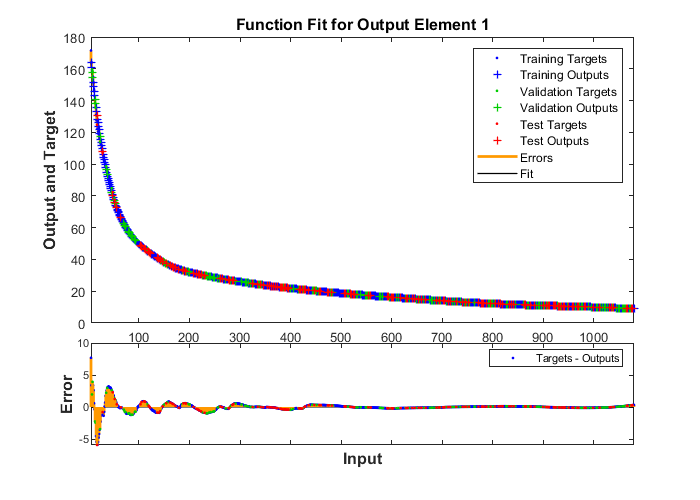
\includegraphics[width=0.74\textwidth]{Textuais/Figuras/NN/tr10-5neuronio.png}
    \fonte{Autores}
    \label{fig:tr10-5n}
\end{figure}

\begin{figure}[h]
    \caption{Curva ajustada para os dados para TR 10 anos e 10 neurônios artificiais}
    \centering
    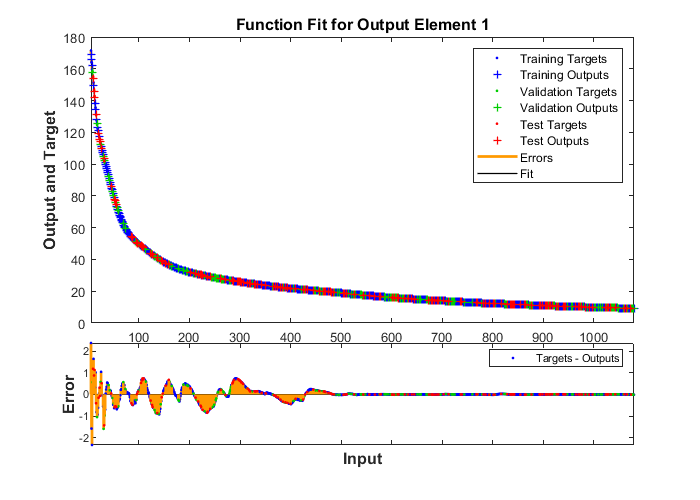
\includegraphics[width=0.74\textwidth]{Textuais/Figuras/NN/tr10-10neuronio.png}
    \fonte{Autores}
    \label{fig:tr10-10n}
\end{figure}
%FIM TR 10

%TR 15
\begin{figure}[h]
    \caption{Curva ajustada para os dados para TR 15 anos e 1 neurônio artificial}
    \centering
    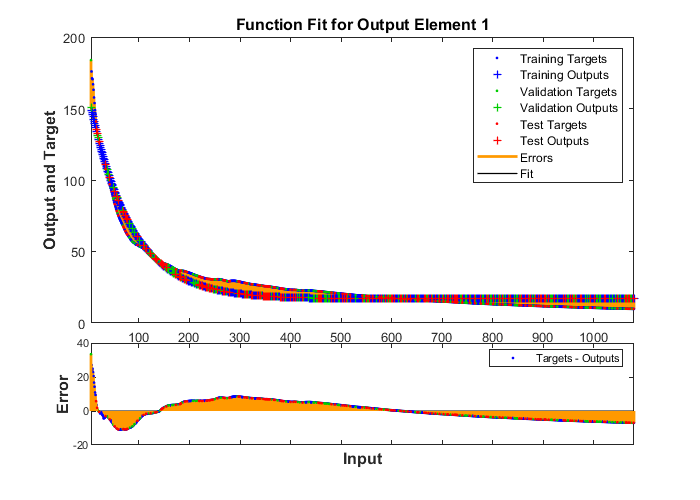
\includegraphics[width=0.74\textwidth]{Textuais/Figuras/NN/tr15-1neuronio.png}
    \fonte{Autores}
    \label{fig:tr15-1n}
\end{figure}

\begin{figure}[h]
    \caption{Curva ajustada para os dados para TR 15 anos e 2 neurônios artificiais}
    \centering
    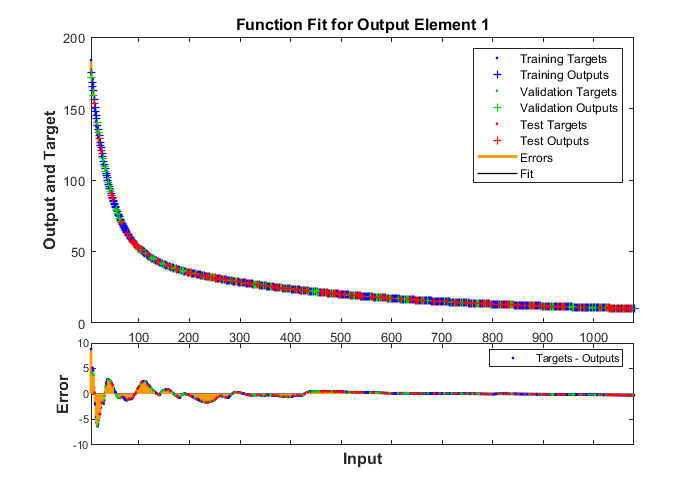
\includegraphics[width=0.74\textwidth]{Textuais/Figuras/NN/tr15-2neuronio.png}
    \fonte{Autores}
    \label{fig:tr15-2n}
\end{figure}

\begin{figure}[h]
    \caption{Curva ajustada para os dados para TR 15 anos e 5 neurônios artificiais}
    \centering
    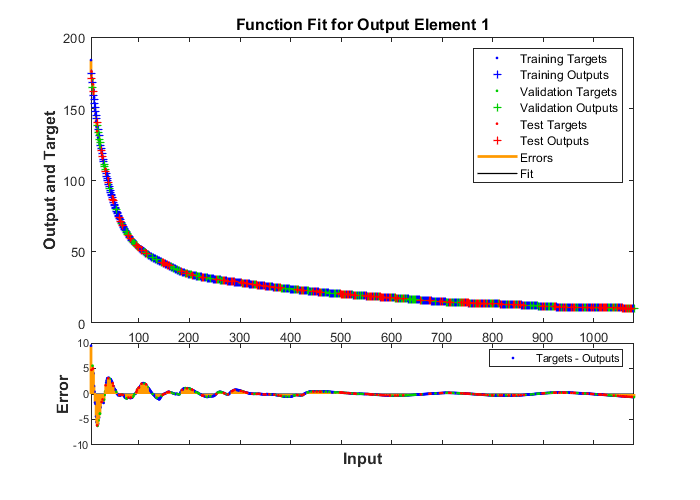
\includegraphics[width=0.74\textwidth]{Textuais/Figuras/NN/tr15-5neuronio.png}
    \fonte{Autores}
    \label{fig:tr15-5n}
\end{figure}

\begin{figure}[h]
    \caption{Curva ajustada para os dados para TR 15 anos e 10 neurônios artificiais}
    \centering
    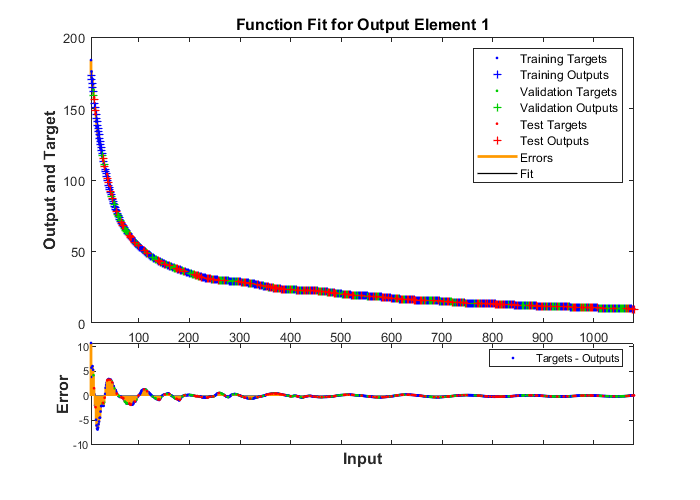
\includegraphics[width=0.74\textwidth]{Textuais/Figuras/NN/tr15-10neuronio.png}
    \fonte{Autores}
    \label{fig:tr15-10n}
\end{figure}
%FIM TR 15

%TR 20
\begin{figure}[h]
    \caption{Curva ajustada para os dados para TR 20 anos e 1 neurônio artificial}
    \centering
    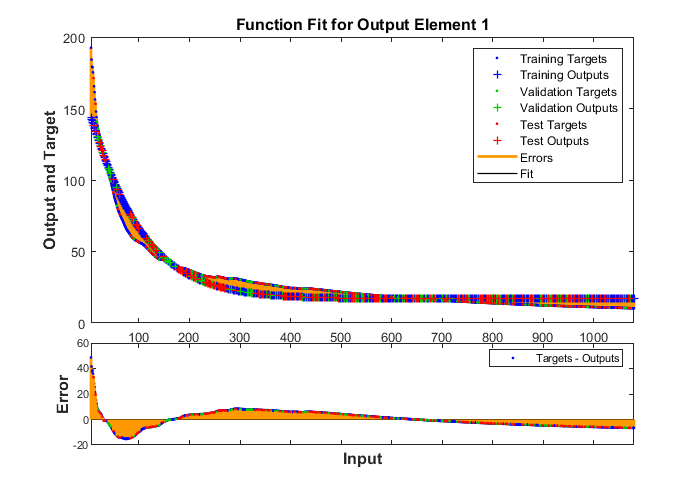
\includegraphics[width=0.74\textwidth]{Textuais/Figuras/NN/tr20-1neuronio.png}
    \fonte{Autores}
    \label{fig:tr20-1n}
\end{figure}

\begin{figure}[h]
    \caption{Curva ajustada para os dados para TR 20 anos e 2 neurônios artificiais}
    \centering
    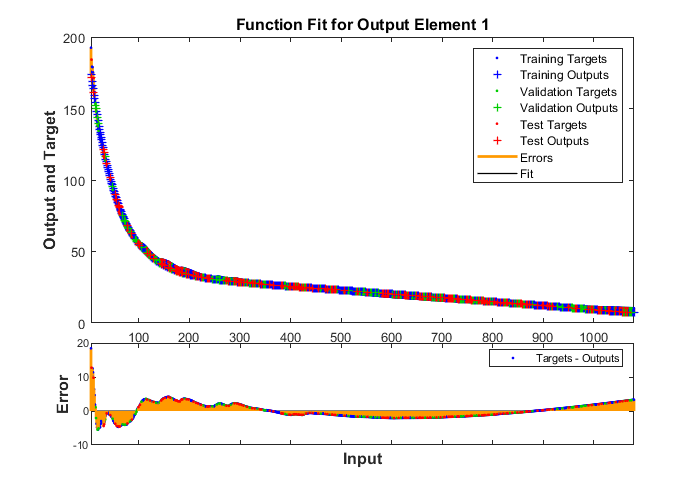
\includegraphics[width=0.74\textwidth]{Textuais/Figuras/NN/tr20-2neuronio.png}
    \fonte{Autores}
    \label{fig:tr20-2n}
\end{figure}

\begin{figure}[h]
    \caption{Curva ajustada para os dados para TR 20 anos e 5 neurônios artificiais}
    \centering
    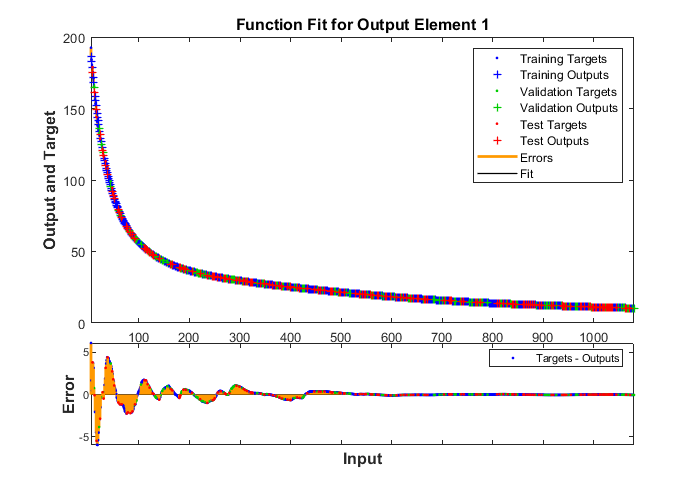
\includegraphics[width=0.74\textwidth]{Textuais/Figuras/NN/tr20-5neuronio.png}
    \fonte{Autores}
    \label{fig:tr20-5n}
\end{figure}

\begin{figure}[h]
    \caption{Curva ajustada para os dados para TR 20 anos e 10 neurônios artificiais}
    \centering
    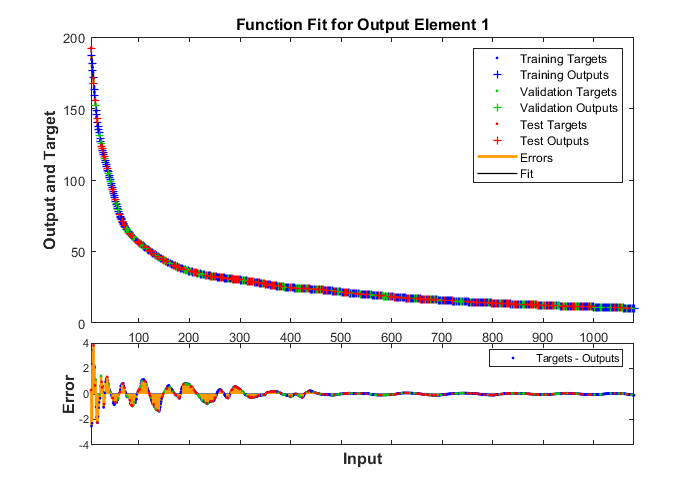
\includegraphics[width=0.74\textwidth]{Textuais/Figuras/NN/tr20-10neuronio.png}
    \fonte{Autores}
    \label{fig:tr20-10n}
\end{figure}
%FIM TR 20

%TR 25
\begin{figure}[h]
    \caption{Curva ajustada para os dados para TR 25 anos e 1 neurônio artificial}
    \centering
    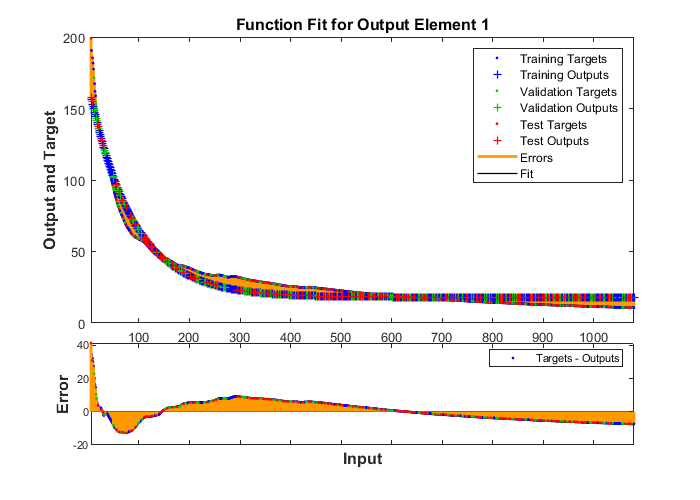
\includegraphics[width=0.74\textwidth]{Textuais/Figuras/NN/tr25-1neuronio.png}
    \fonte{Autores}
    \label{fig:tr25-1n}
\end{figure}

\begin{figure}[h]
    \caption{Curva ajustada para os dados para TR 25 anos e 2 neurônios artificiais}
    \centering
    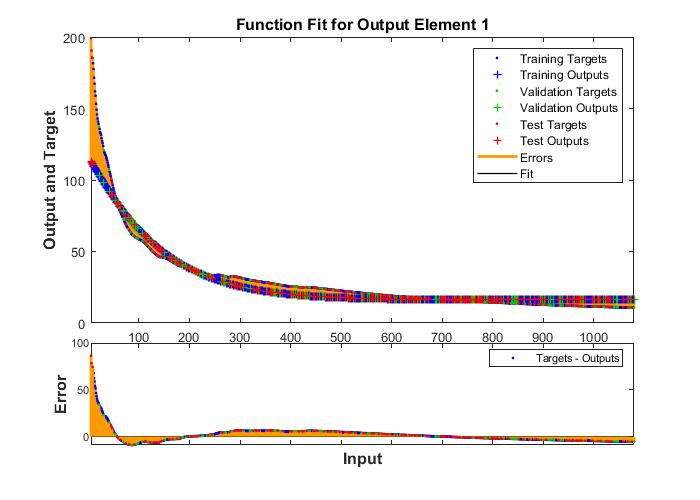
\includegraphics[width=0.74\textwidth]{Textuais/Figuras/NN/tr25-2neuronio.png}
    \fonte{Autores}
    \label{fig:tr25-2n}
\end{figure}

\begin{figure}[h]
    \caption{Curva ajustada para os dados para TR 25 anos e 5 neurônios artificiais}
    \centering
    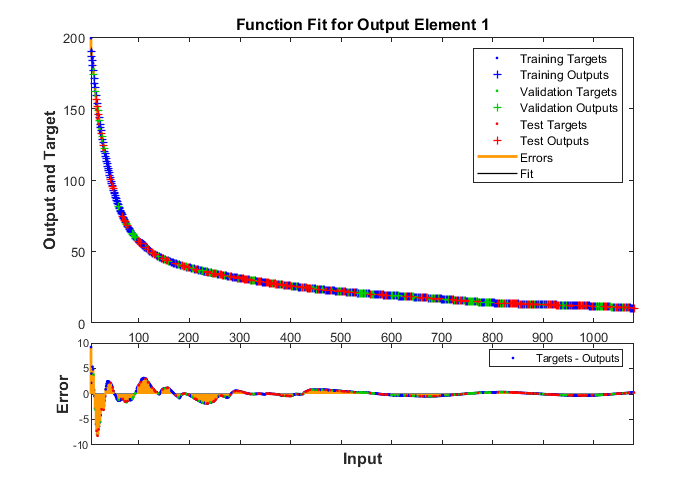
\includegraphics[width=0.74\textwidth]{Textuais/Figuras/NN/tr25-5neuronio.png}
    \fonte{Autores}
    \label{fig:tr25-5n}
\end{figure}

\begin{figure}[h]
    \caption{Curva ajustada para os dados para TR 25 anos e 10 neurônios artificiais}
    \centering
    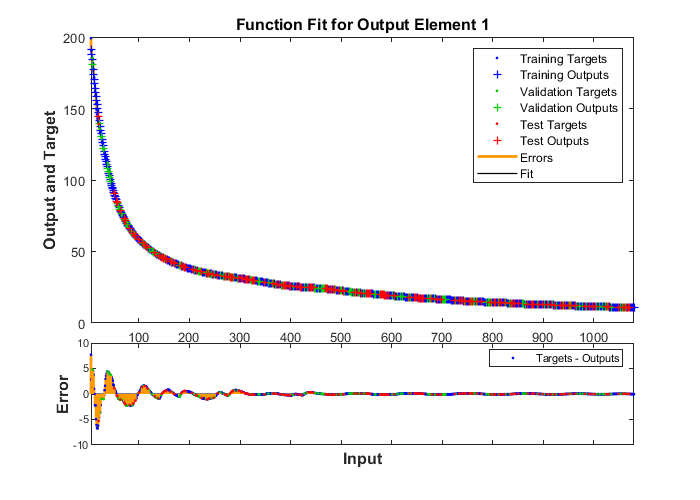
\includegraphics[width=0.74\textwidth]{Textuais/Figuras/NN/tr25-10neuronio.png}
    \fonte{Autores}
    \label{fig:tr25-10n}
\end{figure}
%FIM TR 25

%TR 50
\begin{figure}[h]
    \caption{Curva ajustada para os dados para TR 50 anos e 1 neurônio artificial}
    \centering
    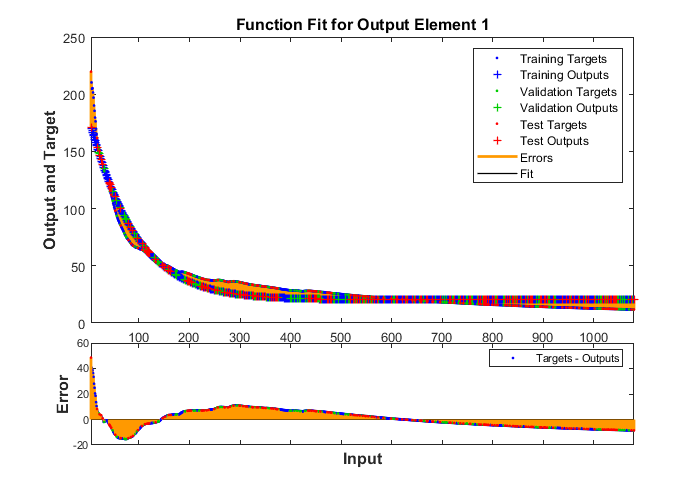
\includegraphics[width=0.74\textwidth]{Textuais/Figuras/NN/tr50-1neuronio.png}
    \fonte{Autores}
    \label{fig:tr50-1n}
\end{figure}

\begin{figure}[h]
    \caption{Curva ajustada para os dados para TR 50 anos e 2 neurônios artificiais}
    \centering
    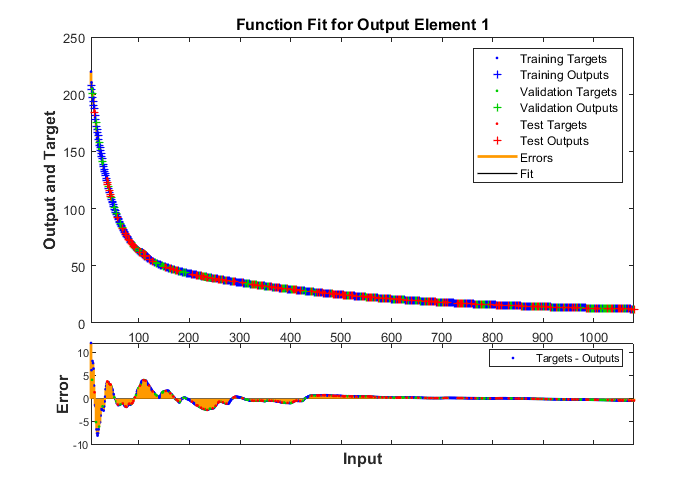
\includegraphics[width=0.74\textwidth]{Textuais/Figuras/NN/tr50-2neuronio.png}
    \fonte{Autores}
    \label{fig:tr50-2n}
\end{figure}

\begin{figure}[h]
    \caption{Curva ajustada para os dados para TR 50 anos e 5 neurônios artificiais}
    \centering
    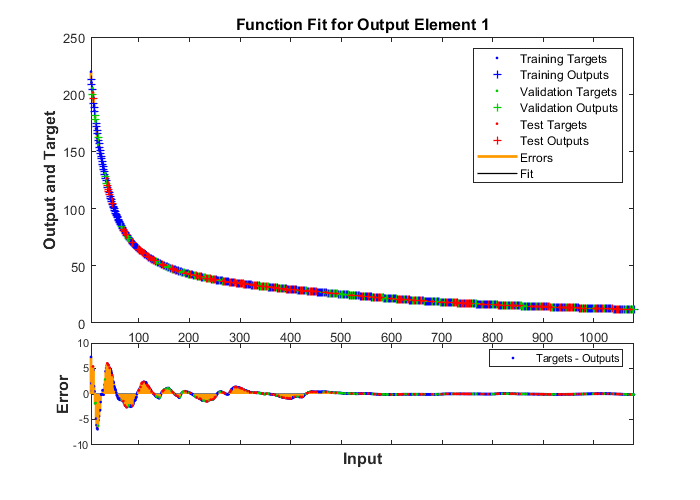
\includegraphics[width=0.74\textwidth]{Textuais/Figuras/NN/tr50-5neuronio.png}
    \fonte{Autores}
    \label{fig:tr50-5n}
\end{figure}

\begin{figure}[h]
    \caption{Curva ajustada para os dados para TR 50 anos e 10 neurônios artificiais}
    \centering
    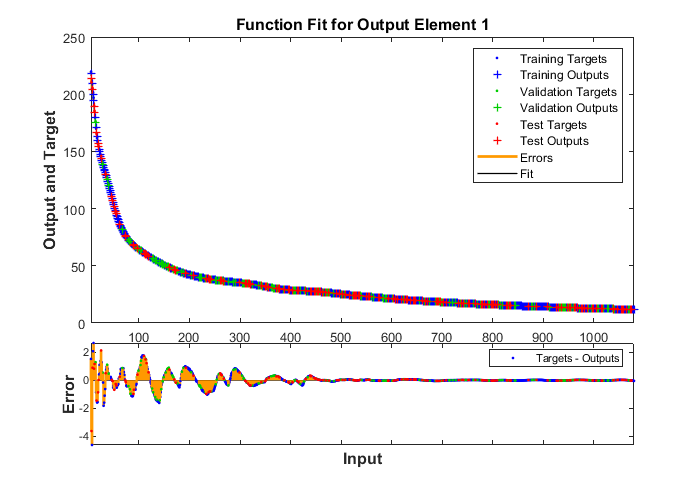
\includegraphics[width=0.74\textwidth]{Textuais/Figuras/NN/tr50-10neuronio.png}
    \fonte{Autores}
    \label{fig:tr50-10n}
\end{figure}
%FIM TR 50

%TR 100
\begin{figure}[h]
    \caption{Curva ajustada para os dados para TR 100 anos e 1 neurônio artificial}
    \centering
    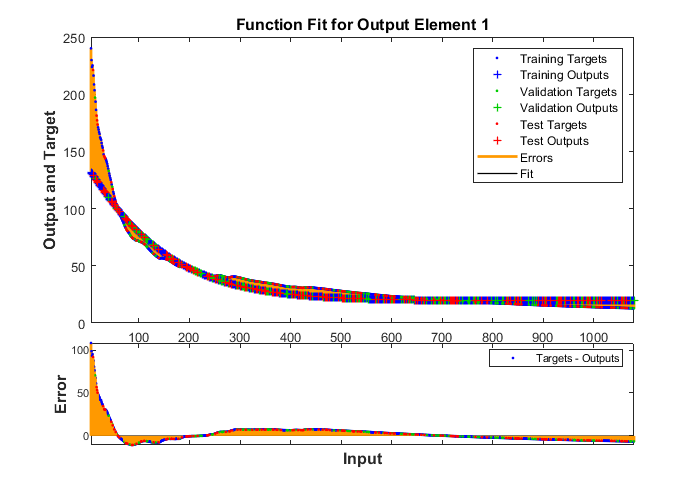
\includegraphics[width=0.74\textwidth]{Textuais/Figuras/NN/tr100-1neuronio.png}
    \fonte{Autores}
    \label{fig:tr100-1n}
\end{figure}

\begin{figure}[h]
    \caption{Curva ajustada para os dados para TR 100 anos e 2 neurônios artificiais}
    \centering
    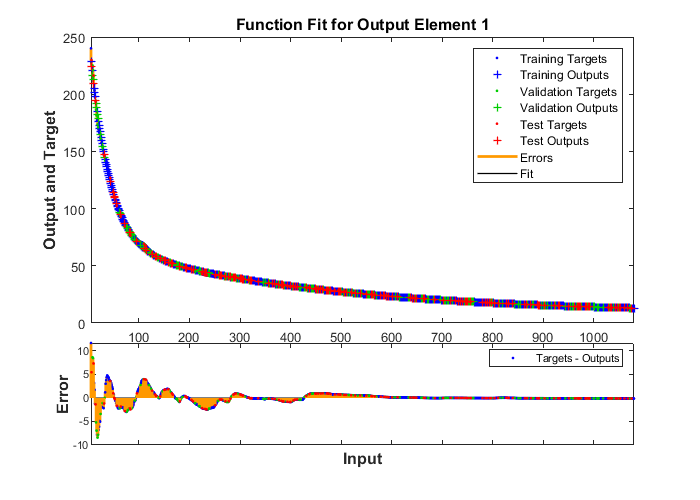
\includegraphics[width=0.74\textwidth]{Textuais/Figuras/NN/tr100-2neuronio.png}
    \fonte{Autores}
    \label{fig:tr100-2n}
\end{figure}

\begin{figure}[h]
    \caption{Curva ajustada para os dados para TR 100 anos e 5 neurônios artificiais}
    \centering
    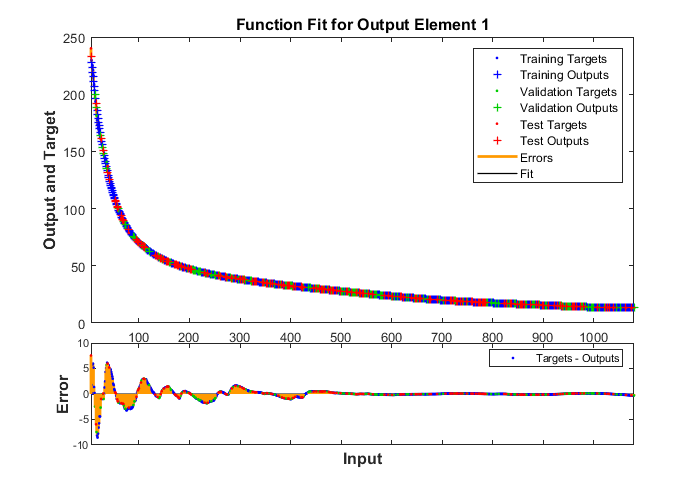
\includegraphics[width=0.74\textwidth]{Textuais/Figuras/NN/tr100-5neuronio.png}
    \fonte{Autores}
    \label{fig:tr100-5n}
\end{figure}

\begin{figure}[h]
    \caption{Curva ajustada para os dados para TR 100 anos e 10 neurônios artificiais}
    \centering
    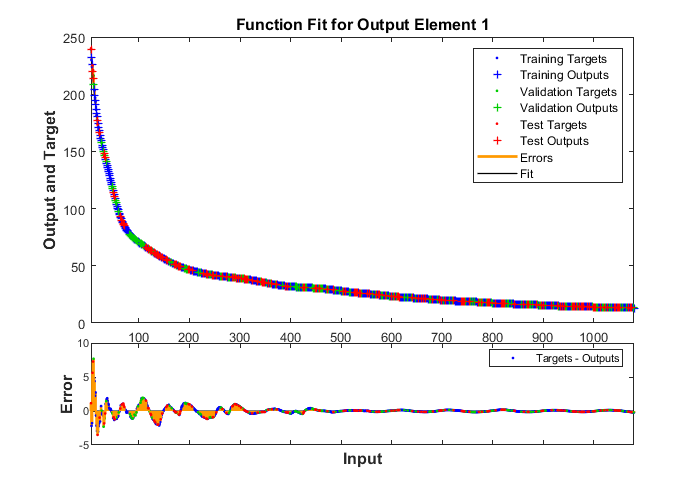
\includegraphics[width=0.74\textwidth]{Textuais/Figuras/NN/tr100-10neuronio.png}
    \fonte{Autores}
    \label{fig:tr100-10n}
\end{figure}
%FIM TR 100

